% Dokumentklassen:
% article, report, beamer, book, letter etc.
% https://en.wikibooks.org/wiki/LaTeX/Document_Structure
\documentclass[a4paper]{article}

% Seitenränder Abstand setzen
\usepackage[margin=80pt]{geometry}

% Deutsches Sprachpaket
\usepackage[ngerman]{babel}
% UTF8 Input Encoding
\usepackage[utf8]{inputenc}

\usepackage{amsmath}
\usepackage{amssymb}

% Schriftbild ändern
% https://en.wikibooks.org/wiki/LaTeX/Fonts
\usepackage[scaled]{helvet}
% (Sans) Serifen oder anderes
% \rmdefault: Serifen
% \sfdefault: Sans-Serifen
% \ttdefault: Typewriter
\renewcommand{\familydefault}{\sfdefault}
% Fontencoding (für ä, ö, ü etc.)
\usepackage[T1]{fontenc}

% Gänsefüsschen richtig kompilieren
\usepackage [autostyle]{csquotes}
\MakeOuterQuote{"}

% Hyperlinks farblos
\usepackage[hidelinks]{hyperref}
\hypersetup{colorlinks=false}

% Package für Aufzählungen
\usepackage{enumitem}
% kein Abstand zwischen Aufzählungen
% Sollen doch Abstände vorhanden sein: nach Aufzählung {itemsep=1em}
\setlist{nosep}

% Grafik-Packages, für Figures, Subfigures und PDF als Import
\usepackage{graphicx}
\usepackage{subcaption}
\usepackage{pdfpages}

% Package und Einstellungen für Java-Code-Darstellung
% Werden erstellt mit \begin{lstlisting}
\usepackage{listings}
\usepackage{color}
\definecolor{dkgreen}{rgb}{0,0.6,0}
\definecolor{gray}{rgb}{0.5,0.5,0.5}
\definecolor{mauve}{rgb}{0.58,0,0.82}
\lstset{frame=tb,
	language=Java,
	aboveskip=3mm,
	belowskip=3mm,
	showstringspaces=false,
	columns=flexible,
	basicstyle={\small\ttfamily},
	numbers=none,
	numberstyle=\tiny\color{gray},
	keywordstyle=\color{blue},
	commentstyle=\color{dkgreen},
	stringstyle=\color{mauve},
	breaklines=true,
	breakatwhitespace=true,
	tabsize=3
}

\title{\textbf{Zusammenfassung DASB} \\
Data Science Basics}
\date{\today}
\author{Maurin D. Thalmann}

\begin{document}
	
	\pagenumbering{gobble}
	\maketitle
	
	\newpage
	\pagenumbering{arabic}
	\tableofcontents
	
	\newpage
	
	\section{Introduction to Data Science}
	
		\subsection{Introductory Stizzle}
		
		\begin{itemize}
			\item More is different - with different quantity comes different quality, although "more" is always dependent on the point of view.
			\item Data volume nowadays is exploding (276.12 billion GB of digital data)
			\item Data Science tries to close the gap between "Data \textit{available} to an organization" and "Percent of data an organization can \textit{process}".
		\end{itemize}
	
		\begin{figure}[htb!]
			\centering
			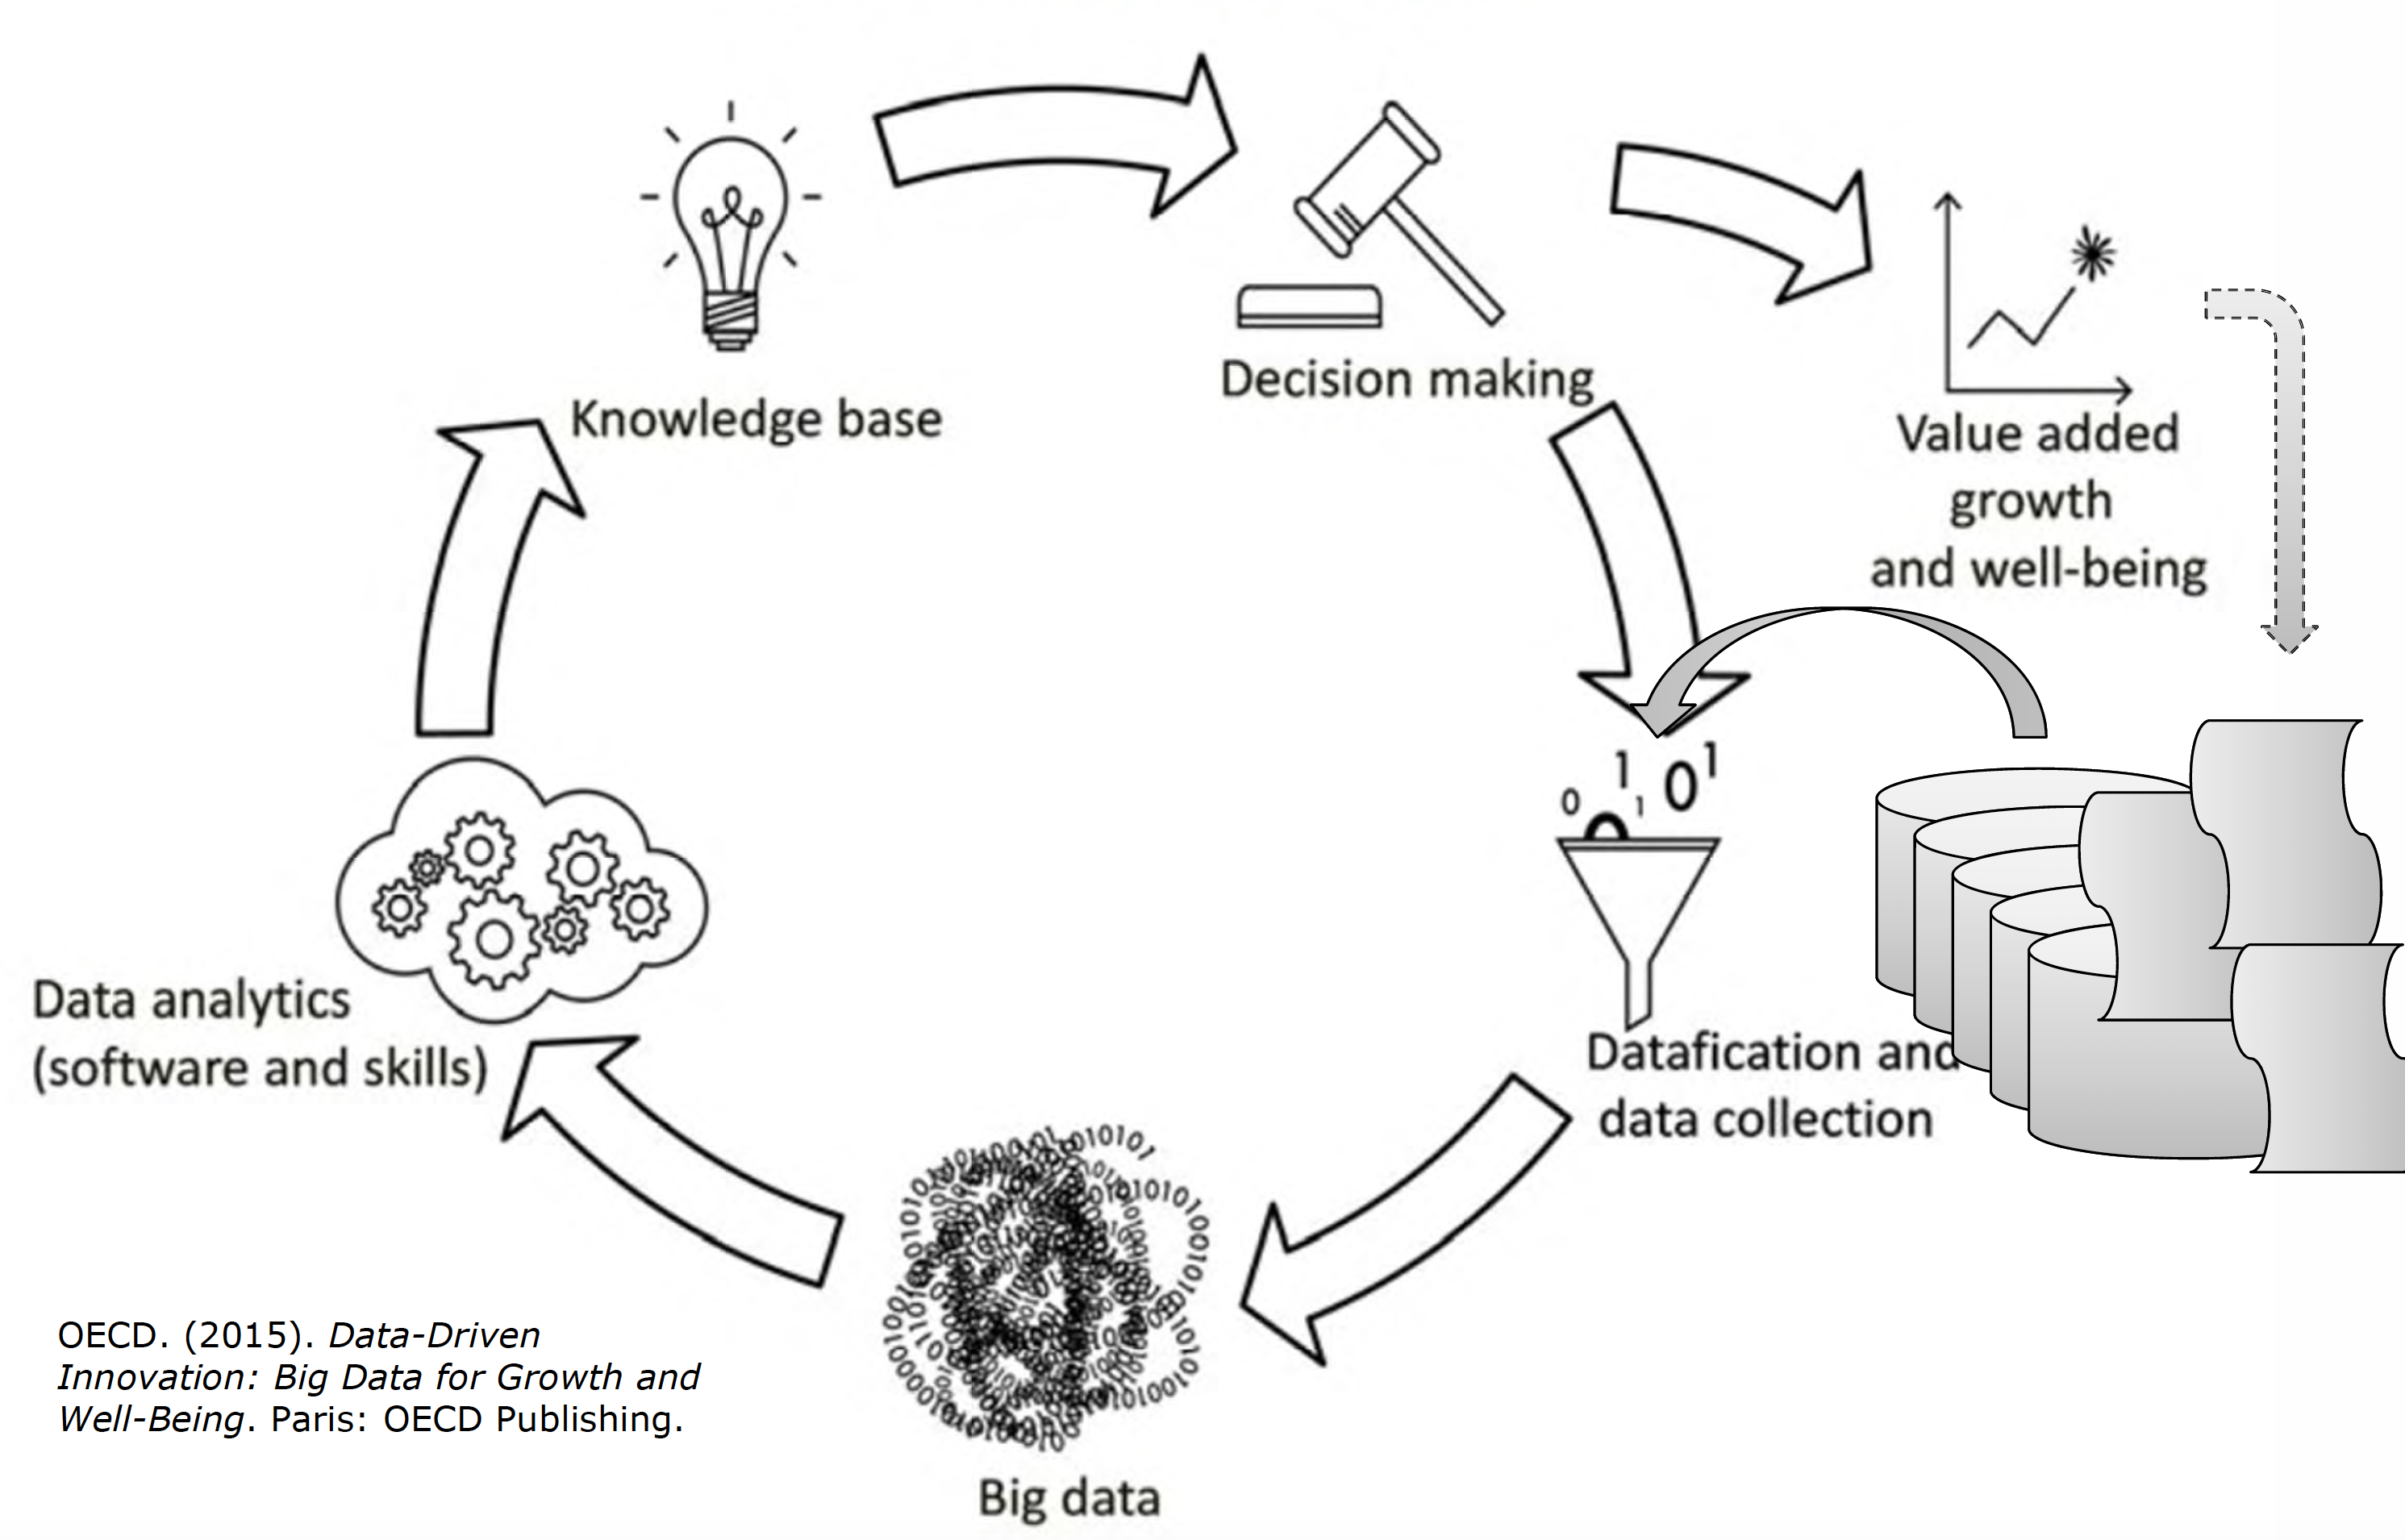
\includegraphics[width=0.5\textwidth]{img/sw01/data_value_cycle.png}
			\caption{Beautiful illustration of the classic data value cycle}
		\end{figure}
	\noindent
		"\textbf{Data Science} is the extraction of actionable knowledge directly from data through a discovery, or hypothesis formulation and hypothesis testing".
		Data Scientists generate knowledge from big data.
		
		\begin{figure}[htb!]
			\centering
			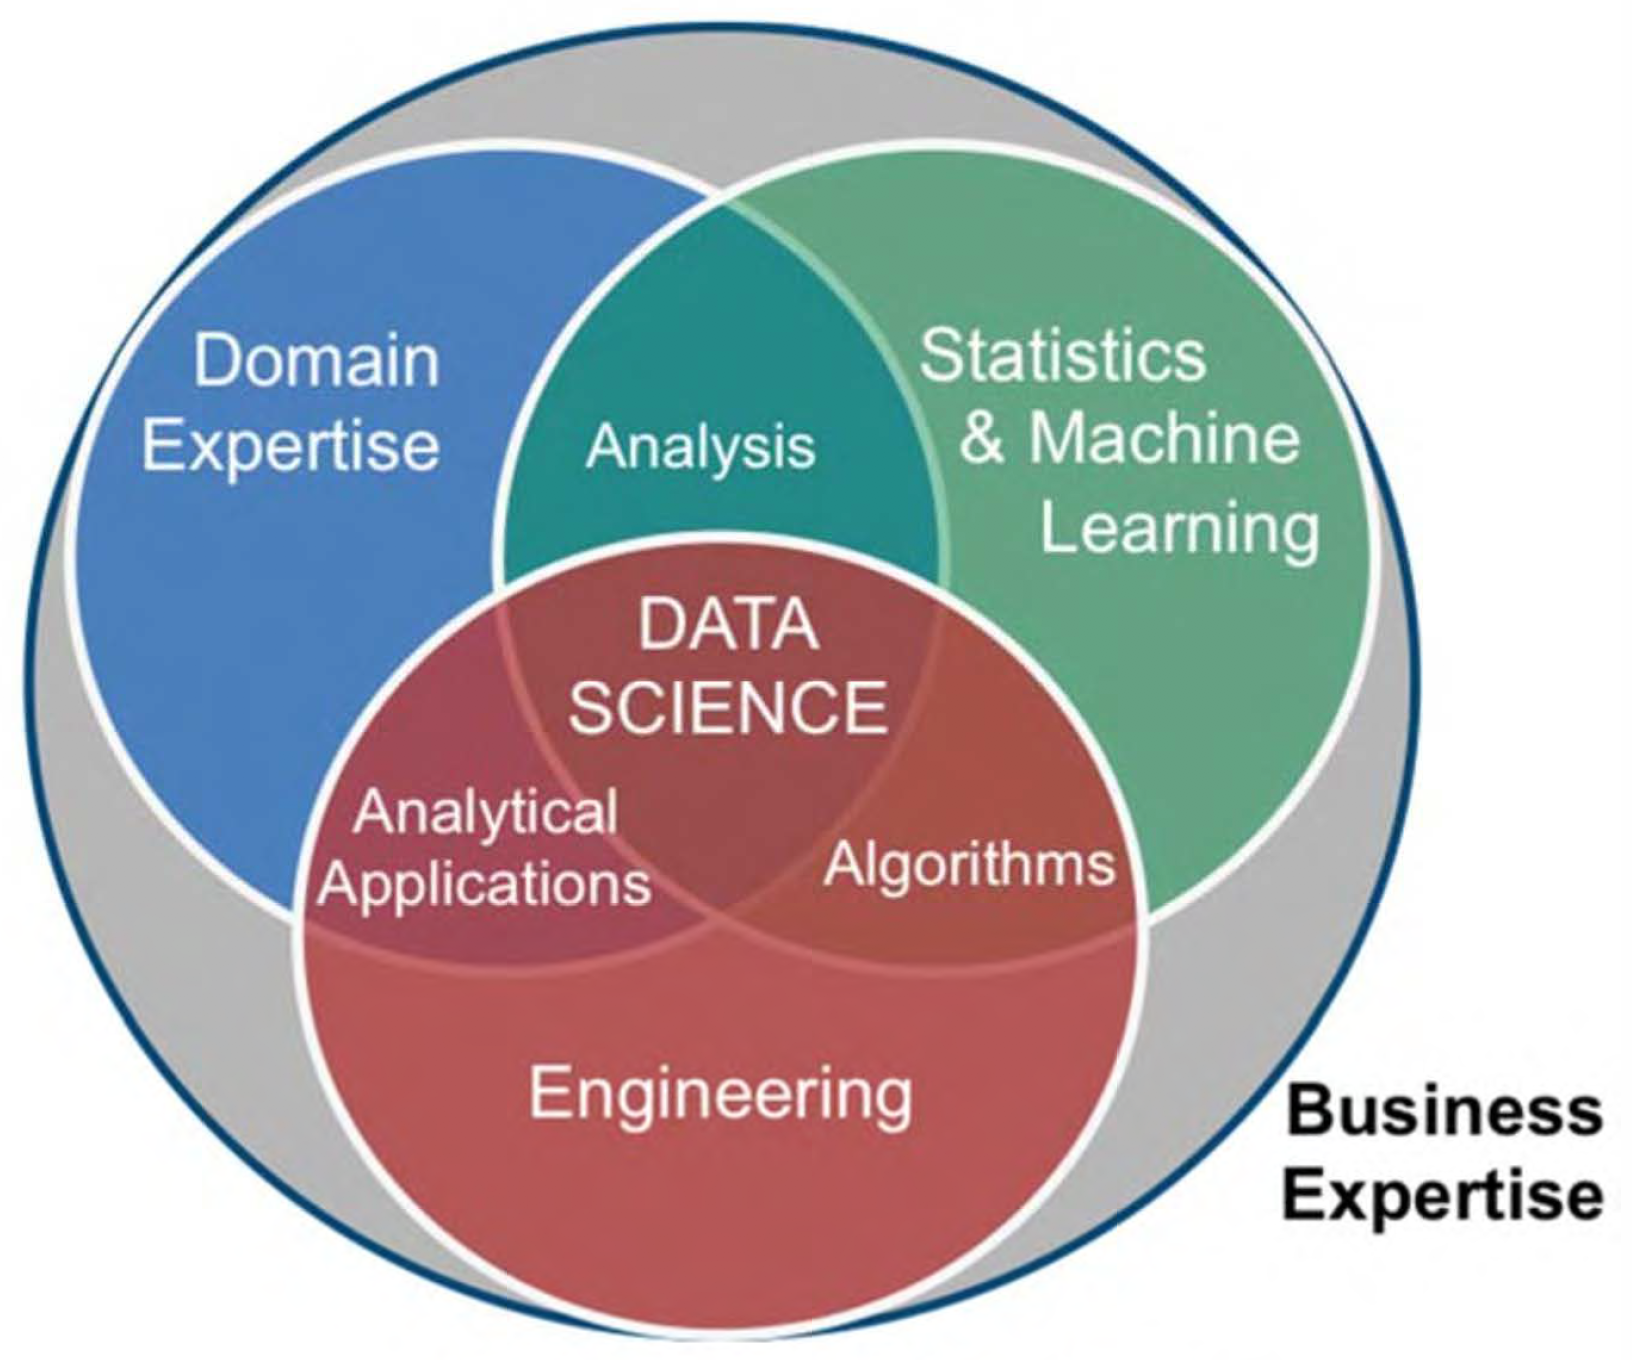
\includegraphics[width=0.3\textwidth]{img/sw01/ds_skills.png}
			\caption{Skills needed in Data Science}
		\end{figure}
	
		\subsection{A Global View on Data Science}
		
		\begin{figure}[htb!]
			\centering
			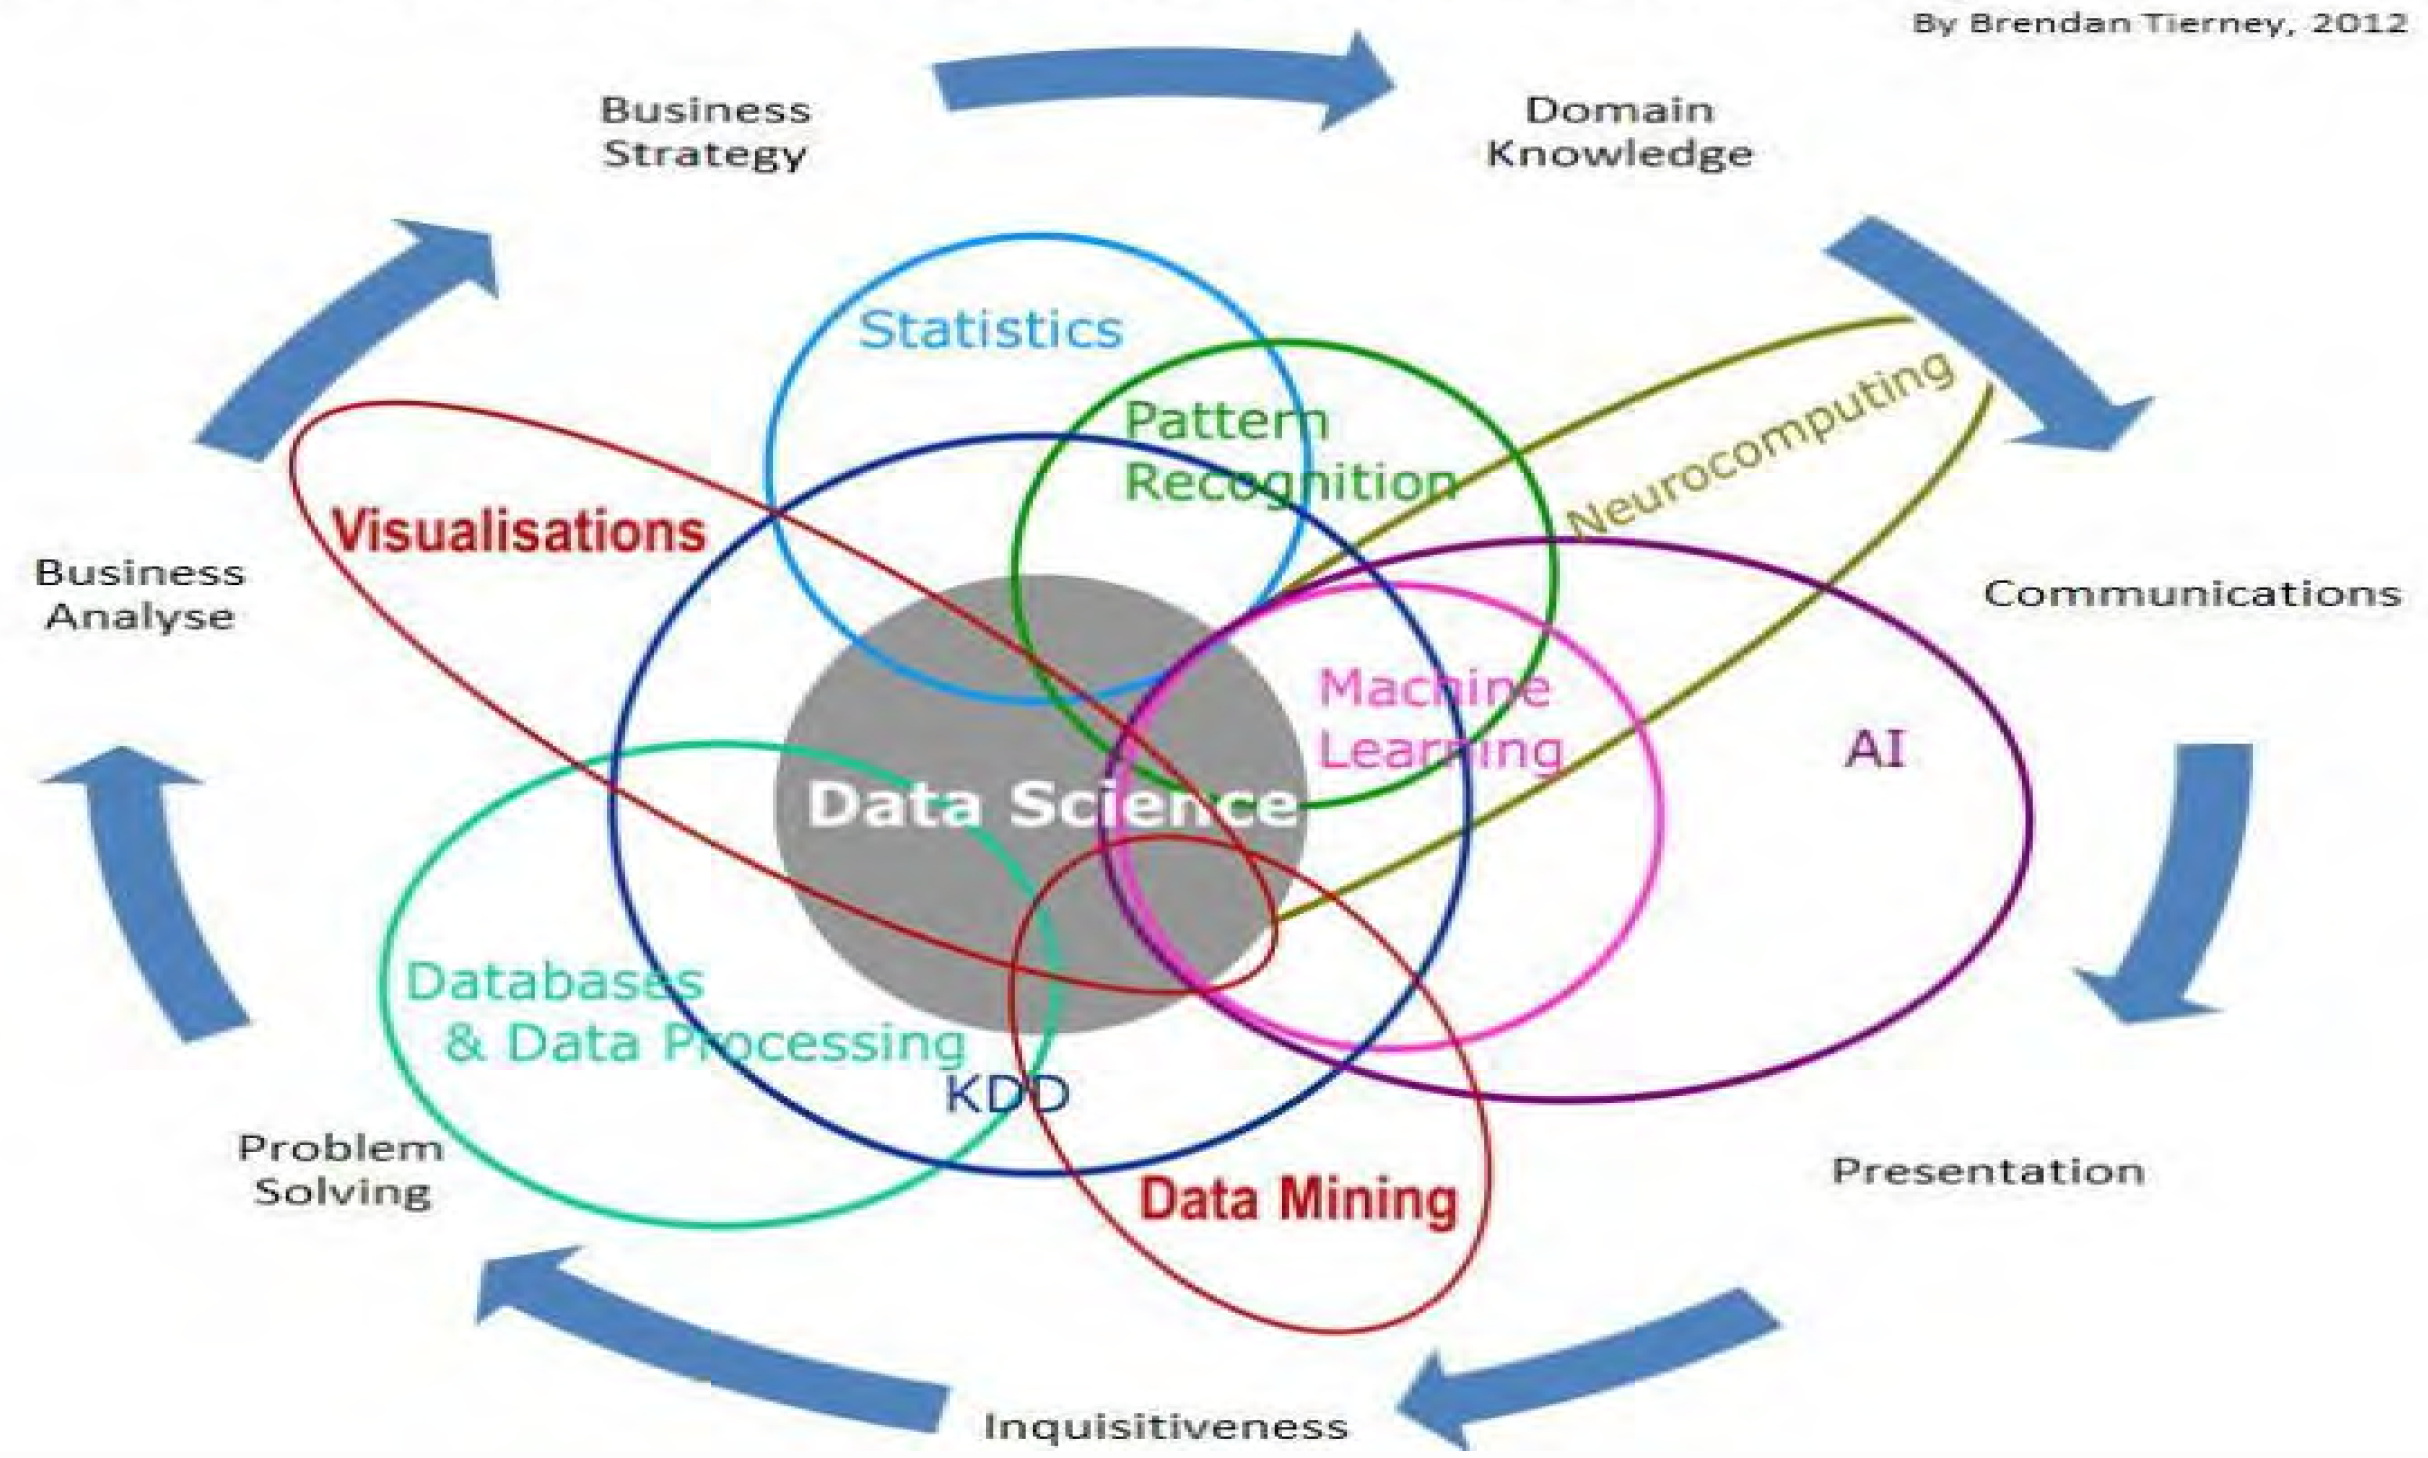
\includegraphics[width=0.5\textwidth]{img/sw01/multidisc.png}
			\caption{Data Science is multidisciplinary}
		\end{figure}
	
		\newpage
		
		\begin{itemize}
			\item \textbf{AI}: programs that perform tasks resembling humans (learn and reason)
			\item \textbf{ML}: algorithms to learn from that data without explicit programming
			\item \textbf{DL}: subset of ML using artificial neural networks for treating vast amount of data (big data)
			\item \textbf{Data Science}: spans the collection, management, analysis and interpretation of large amounts of data with a wide range of applications $\rightarrow$
				make informed decisions based on what was learned
			\item \textbf{EDA} (exploratory data analysis): extract insight from data (outside AI, human based)
		\end{itemize}
	
		\begin{figure}[htb!]
			\centering
			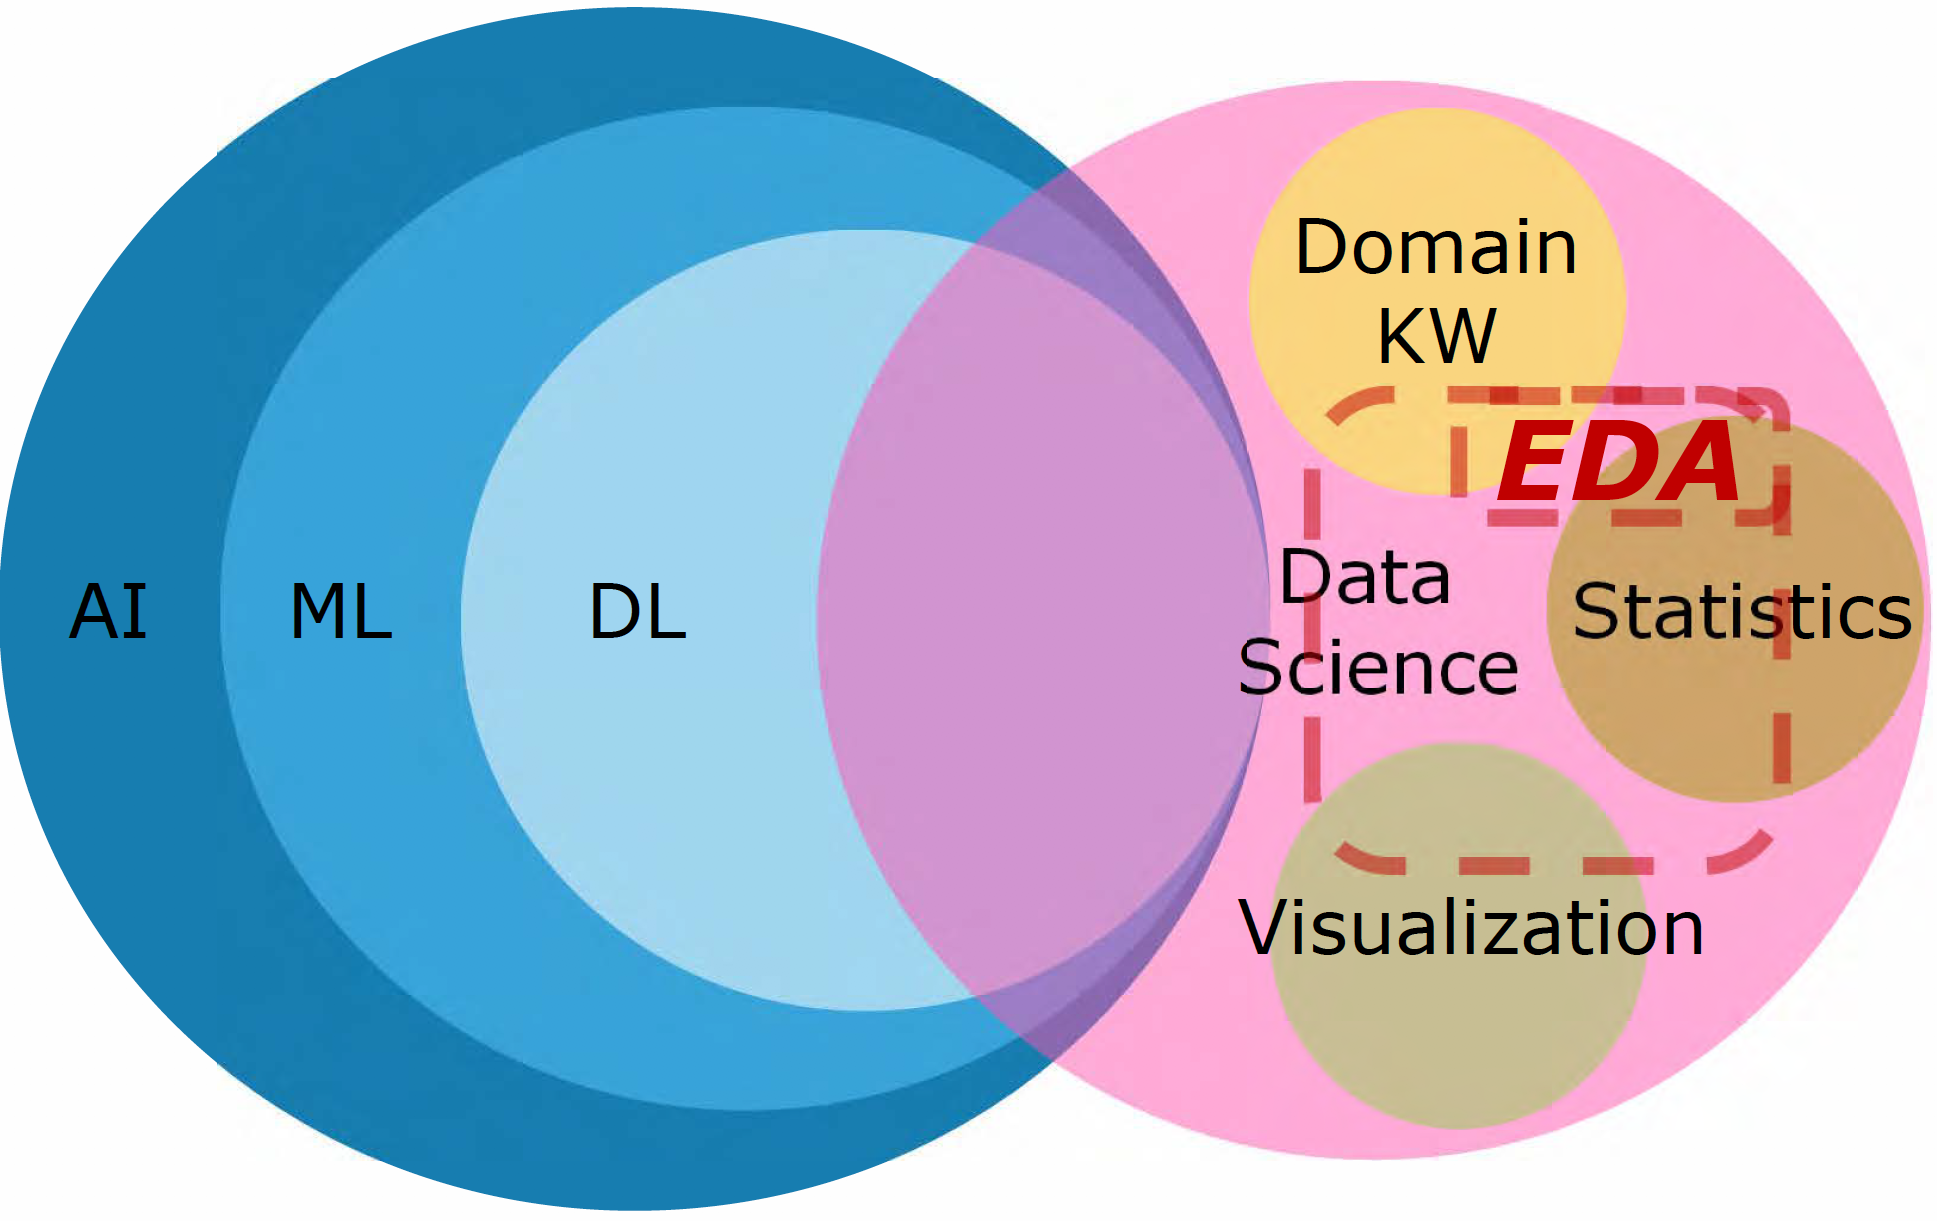
\includegraphics[width=0.4\textwidth]{img/sw01/global_view.png}
			\caption{AI / ML / DL and Data Science}
		\end{figure}
	
		\subsection{Different Concepts in Data Analytics}
		
			\subsubsection{1993 - Online Analytical Processing (OLAP)}
			
			\begin{minipage}[c]{0.3\textwidth}
				\centering
				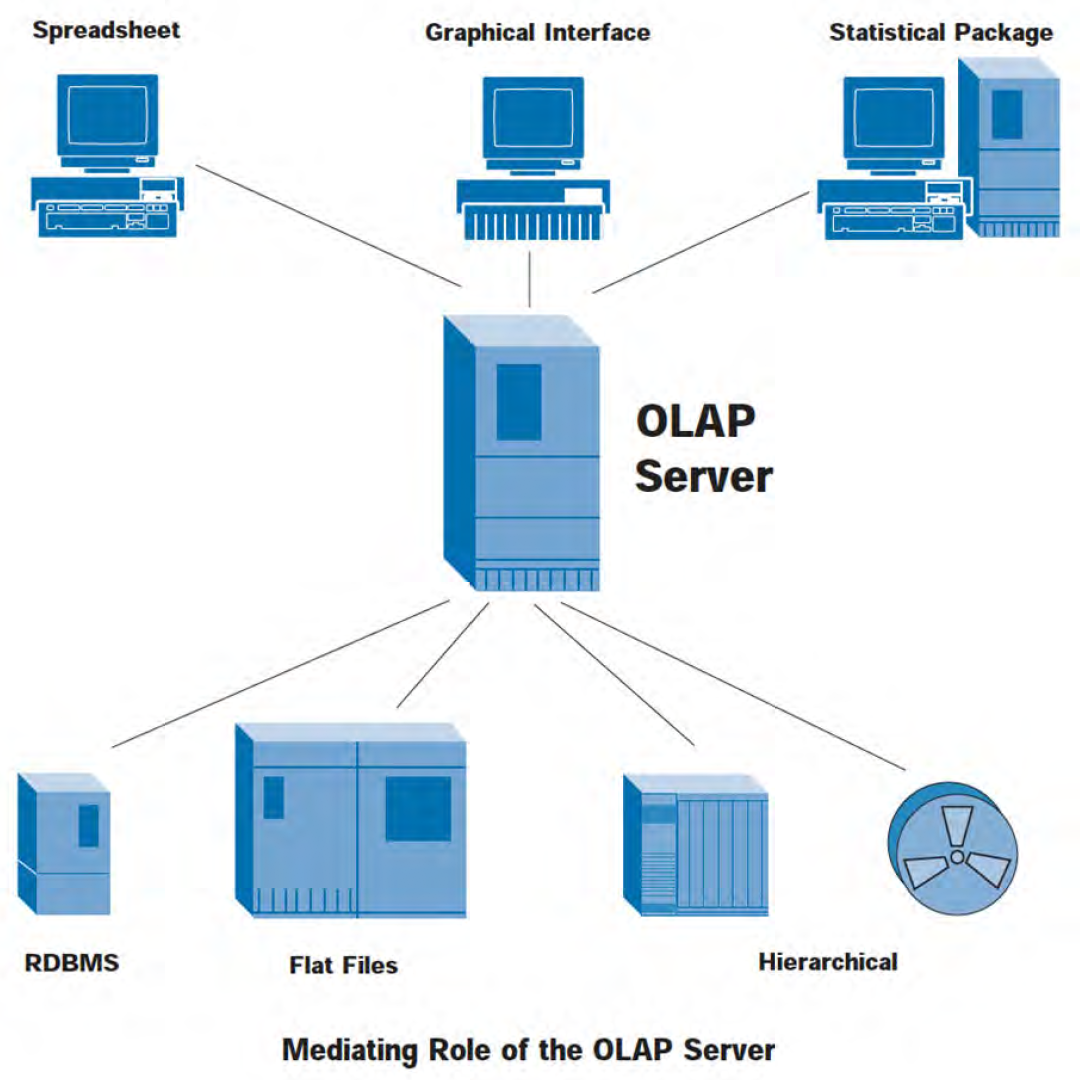
\includegraphics[width=\textwidth]{img/sw01/olap.png}
			\end{minipage}
			\hfill
			\begin{minipage}[c]{0.6\textwidth}
				\begin{itemize}
					\item It's online, not batch (interactive, not programmed in COBOL)
					\item The OLAP system should access the data required to perform the indicated analysis
					\item OLAP tools empower useranalysts to earily perform multi-dimensional analysis, which previously have been avoided because of their perceived complexity.
				\end{itemize}
			\end{minipage}
		
			\subsubsection{1998 - Fuzzy Data Analysis}
			
			\begin{minipage}[c]{0.3\textwidth}
				\centering
				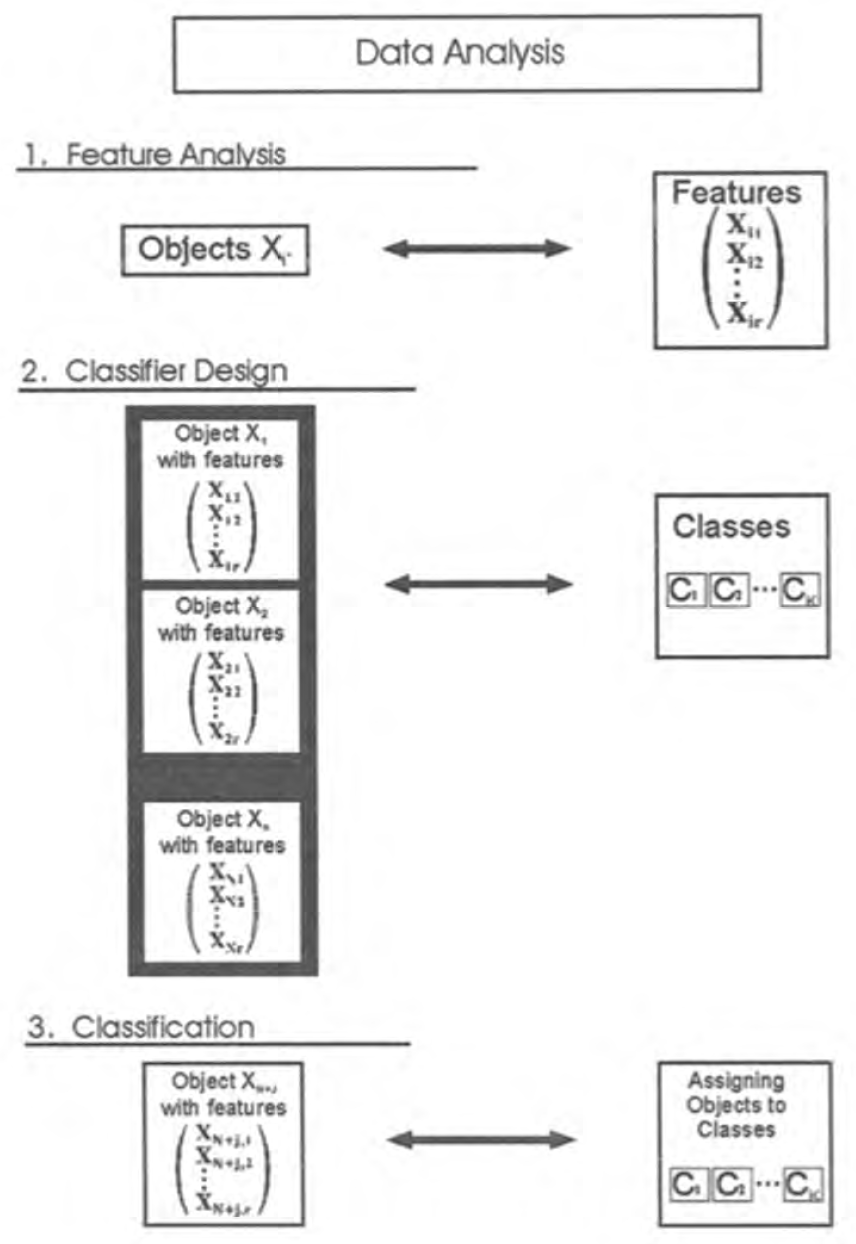
\includegraphics[width=.8\textwidth]{img/sw01/fda.png}
			\end{minipage}
			\hfill
			\begin{minipage}[c]{0.6\textwidth}
				\begin{itemize}
					\item Data analysis can be defined as  \\
						\textbf{search for structure} in data
					\item In data analysis, objects are considered which are described by some attributes
					\item Most of the traditional methods for data analysis assume that patterns to be detected are two-valued
					\item Whenever this is not the case, the relationship between data and classes becomes gradual \\
						$\rightarrow$ Fuzzy Classification
				\end{itemize}
			\end{minipage}
			
			\newpage
			
			\subsubsection{2005 - Data Mining}
			
			\begin{minipage}[c]{0.3\textwidth}
				\centering
				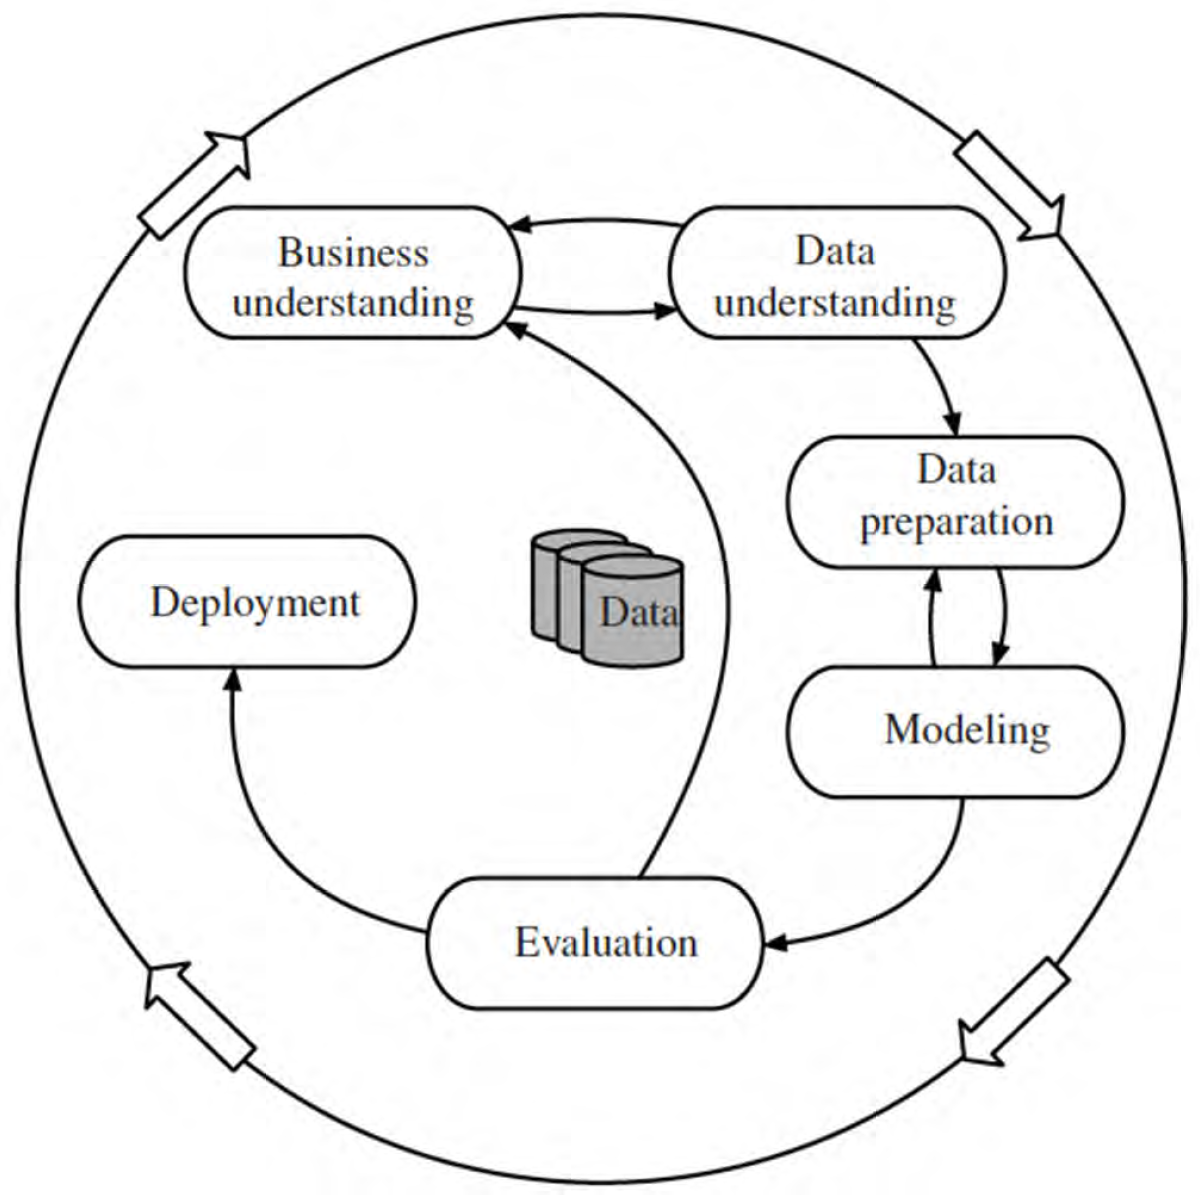
\includegraphics[width=\textwidth]{img/sw01/data-mining.png}
			\end{minipage}
			\hfill
			\begin{minipage}[c]{0.6\textwidth}
				\begin{itemize}
					\item Very similar concept to data science
					\item Machine Learning (modeling) is the technical core of practical data mining applications
					\item Data \textit{Mining} is a business process related to \textit{value} (finding the metaphorical gold nugget)
					\item The lifecycle of a data mining project is defined by the CRISP-DM reference model
				\end{itemize}
			\end{minipage}
		
			\subsubsection{2013 - Predictive Modeling}
			
			\begin{minipage}[c]{0.45\textwidth}
				\centering
				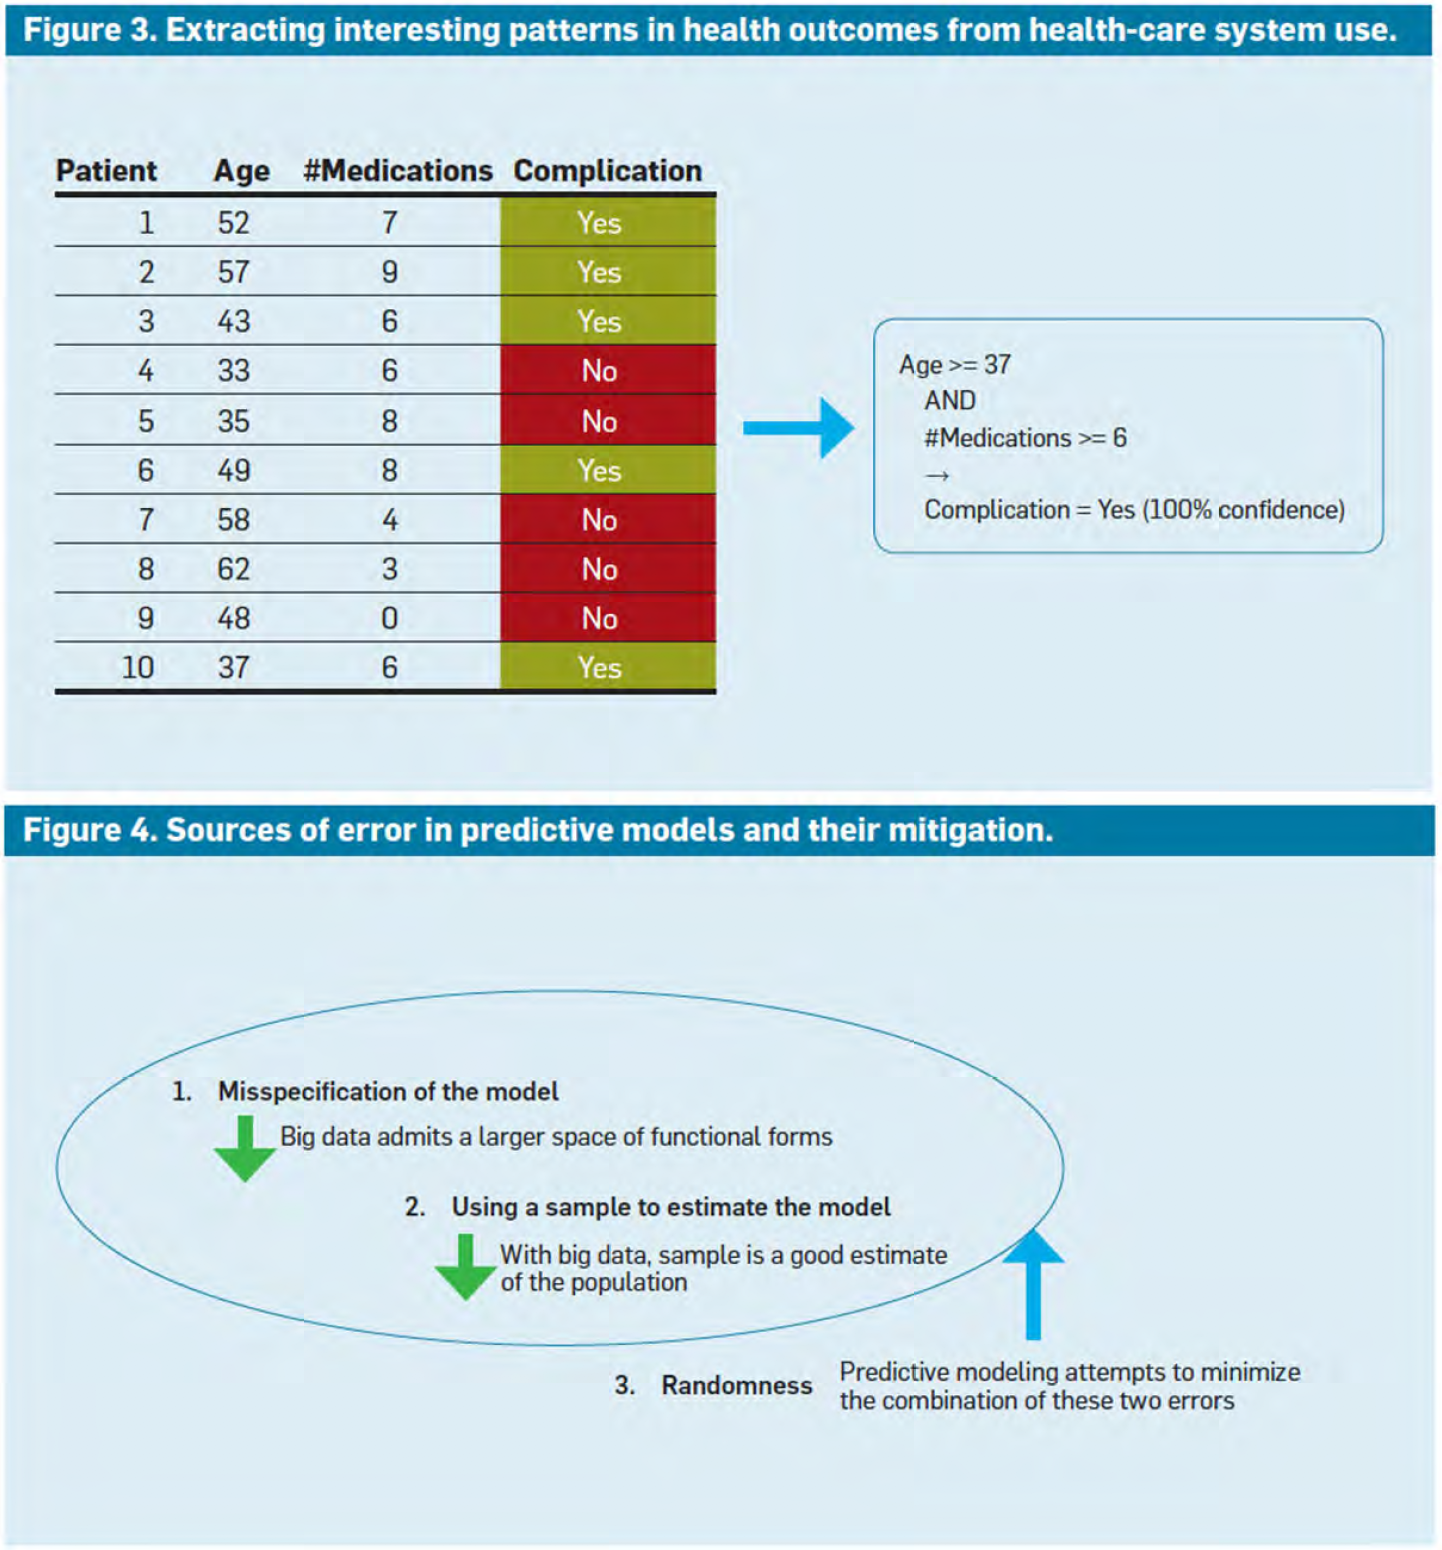
\includegraphics[width=\textwidth]{img/sw01/pred_mod.png}
			\end{minipage}
			\hfill
			\begin{minipage}[c]{0.45\textwidth}
				\begin{itemize}
					\item A common epistemic requirement in assessing whether new knowledge is actionable for decision making in its \textit{predictive power}, not just its ability to explain the past.
					\item The requirement on predictive accuracy on observations that will occur in the future is a key consideration in data science.
				\end{itemize}
			\end{minipage}
		
			\subsubsection{2013 - Data Driven Decision Making}
			
			\begin{minipage}[c]{0.3\textwidth}
				\centering
				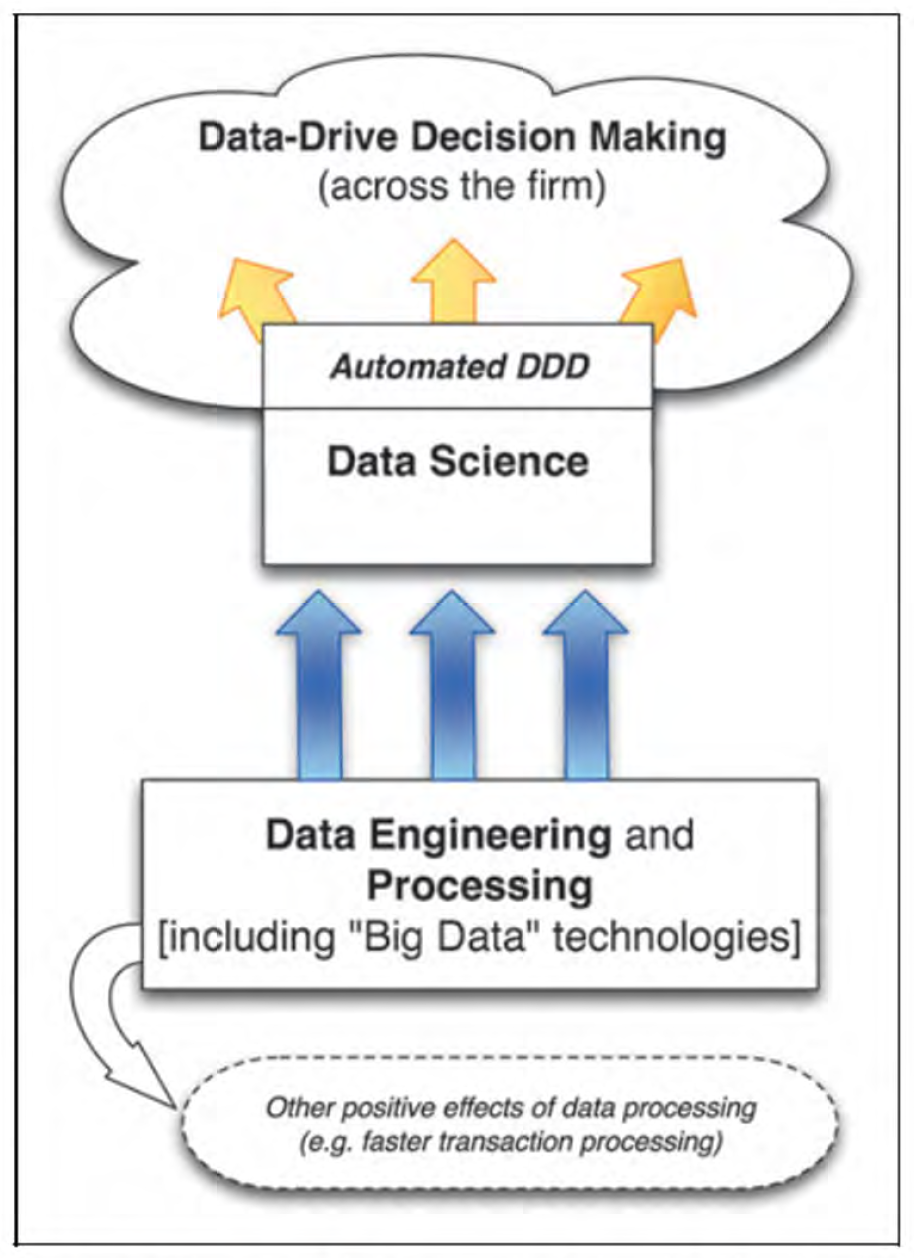
\includegraphics[width=\textwidth]{img/sw01/data_driven.png}
			\end{minipage}
			\hfill
			\begin{minipage}[c]{0.6\textwidth}
				\begin{itemize}
					\item Data science involves much more than just data-mining algorithms.
					\item Successful data scientists must be able to view business problems form a \textit{data perspective}.
				\end{itemize}
			\end{minipage}
		
			\newpage
		
	\section{Intro to R and Exploratory Data Analysis (EDA)}
	
		\subsection{Intro to R}
		
		
		
	
	
	
\end{document}
